\section*{ROLL DECAY TEST}\label{roll-decay-test}

    A common way to determine the roll damping of a ship is to conduct a
roll decay test. The initial heel angle during this test gives the ship
potential energy that subsequently is shifting to kinetic energy as the
ship starts to oscillate during the inital phase of the roll decay test.
The energy is transfered between kinetic and potential energy during the
oscillations. The ship loses energy over time due to the damping as
shown in this illustration:
 
            
    
    \begin{figure}[H]
        \begin{center}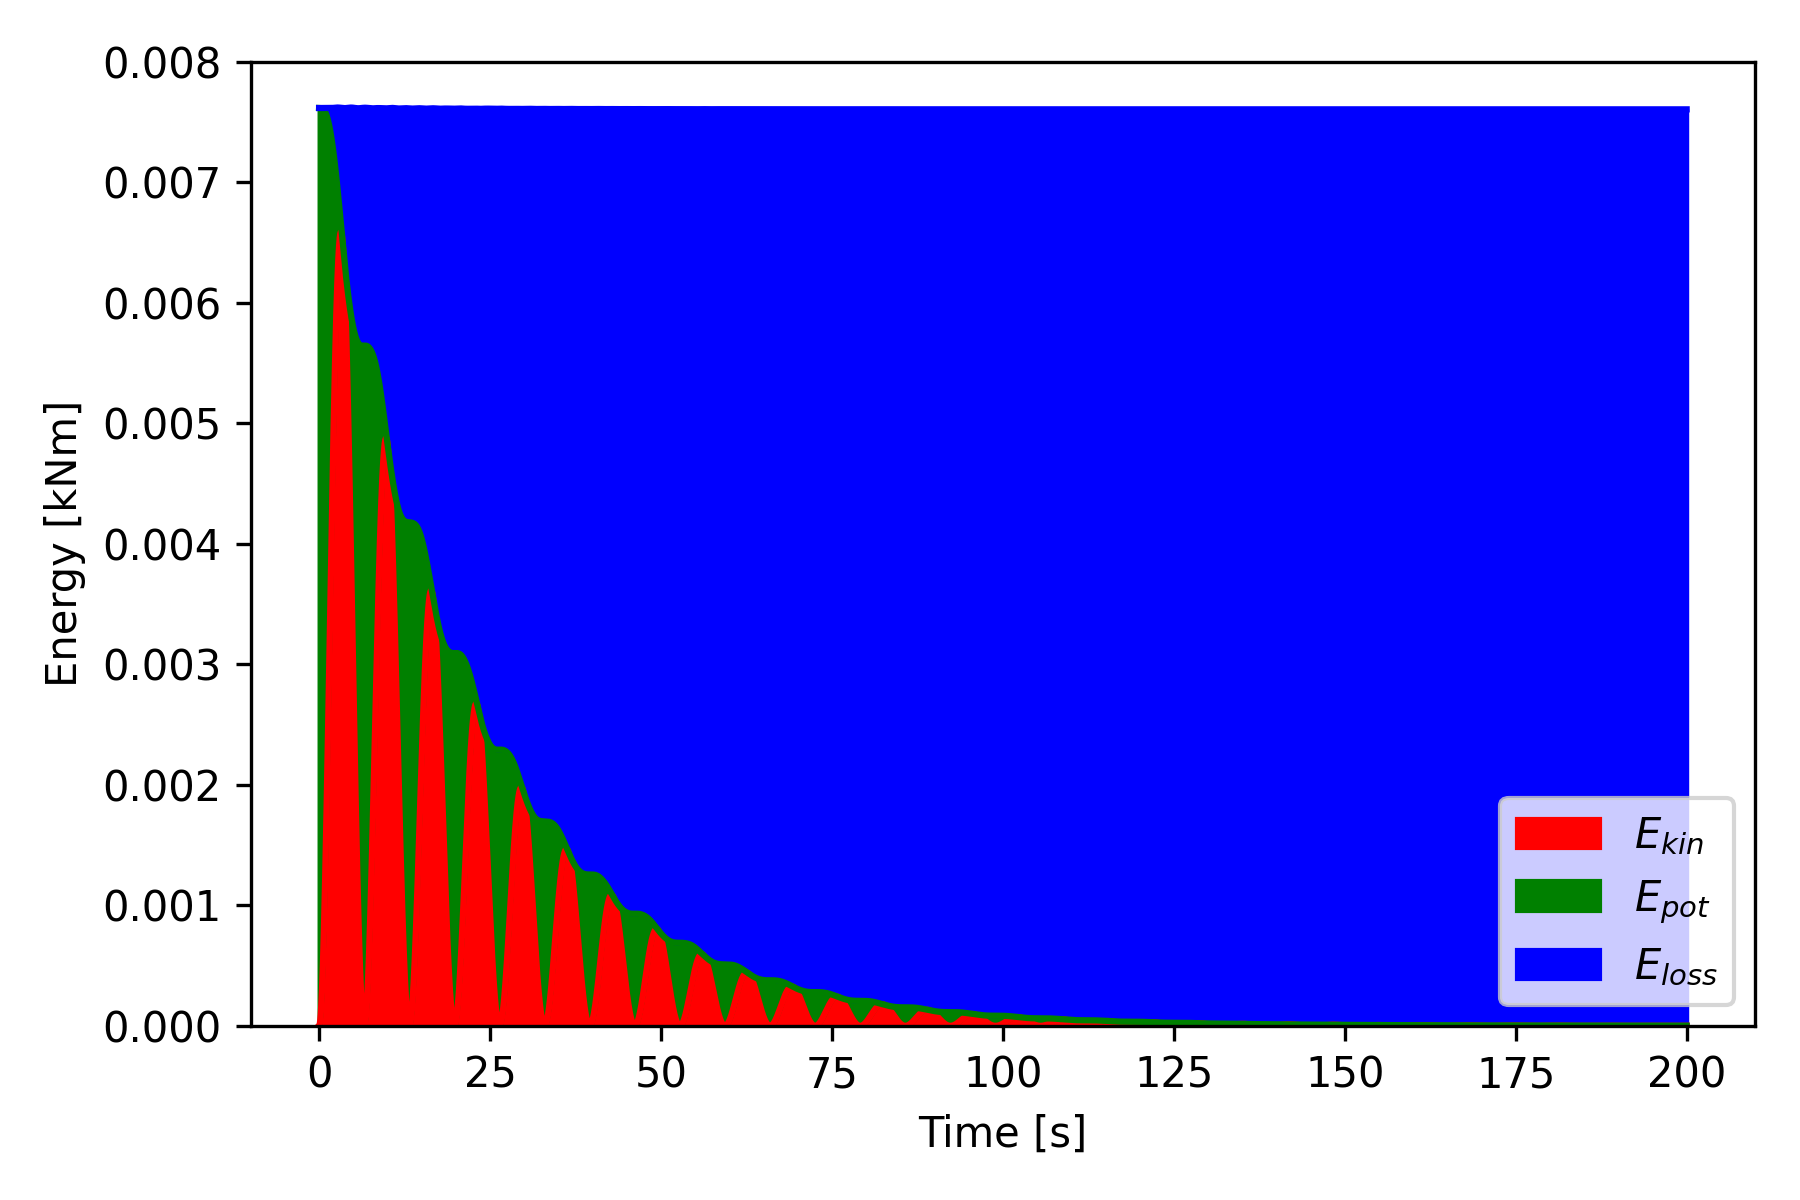
\includegraphics[width = 0.5\textwidth]{figures/energy.png}\end{center}
        \vspace{-1cm}
        \caption{Energy transfer during roll decay}
        \label{fig:energy}
    \end{figure}
    

    Time traces of the roll motion from roll decay tests in model scale
experiments as well as from FNPF and hybrid method simulations are used
in this paper to determine the roll damping. Two different techniques to
identify the damping from these tests are used: the PIT method,
described in the next section and the logartithmic decrement method as
described in \cite{7505983/BYNJ8CFG}.
    \subsection*{PIT method to estimate
damping}\label{pit-method-to-estimate-damping}

    A parameters identification technique (PIT) similar to
\cite{7505983/EXYJELCU} is used to obtain the damping coefficients from
the roll decay tests. In this technique, parameters in a mathematical
model are determined in order to get the best fit to a roll decay time
signal. A derivation of a matematical model suitable for this study is
described below together with a description of how the parameters:
damping, stiffness and inertia coefficients are determined. The roll
decay motion can be expressed in general form according to
\cite{7505983/FB64RGPF}:
 
            
    
    \begin{equation}
A_{44} \ddot{\phi} + \operatorname{B_{44}}\left(\dot{\phi}\right) + \operatorname{C_{44}}\left(\phi\right) = 0
\label{eq:equation}
\end{equation}

    

    Where $B_{44}(\dot{\phi})$ and $C_{44}(\phi)$ are the damping and
stiffness models. A cubic model can be obtained by using cubic damping
and stiffness models:
 
            
    
    \begin{equation}
\operatorname{B_{44}}\left(\dot{\phi}\right) = B_{1} \dot{\phi} + B_{2} \left|{\dot{\phi}}\right| \dot{\phi} + B_{3} \dot{\phi}^{3}
\label{eq:equation}
\end{equation}

    
 
            
    
    \begin{equation}
\operatorname{C_{44}}\left(\phi\right) = C_{1} \phi + C_{3} \phi^{3} + C_{5} \phi^{5}
\label{eq:equation}
\end{equation}

    

    The total equation is then written:
 
            
    
    \begin{equation}
\begin{aligned}
A_{44} \ddot{\phi} + \left(B_{1} + B_{2} \left|{\dot{\phi}}\right| + B_{3} \dot{\phi}^{2}\right) \dot{\phi} \\ + \left(C_{1} + C_{3} \phi^{2} + C_{5} \phi^{4}\right) \phi = 0
\end{aligned}
\label{eq:equation}
\end{equation}

    

    This mathematical model can be reduced to a quadratic damping model when
$B_3=0$ and a linear model when $B_2=B_3=0$. This equation does not
have one unique solution however. If all parameters would be multiplied
by a factor $k$ these parameters would also yield as a solution to the
equation. All parameters are therefore divided by the total inertia
$A_{44}$ (including added mass inertia), replacing the parameters with
new parameters such as: $B_{1A} = B_1/A_{44}$. The equation is now
rewritten with these new parameters which have unique solutions:
 
            
    
    \begin{equation}
\begin{aligned}
\left(B_{1A} + B_{2A} \left|{\dot{\phi}}\right| + B_{3A} \dot{\phi}^{2}\right) \dot{\phi} \\ + \left(C_{1A} + C_{3A} \phi^{2} + C_{5A} \phi^{4}\right) \phi + \ddot{\phi} = 0
\end{aligned}
\label{eq:equation}
\end{equation}

    

    The parameters of this equation can be identified using least square fit
if the time signals $\phi(t)$, $\dot{\phi}(t)$ and
$\ddot{\phi}(t)$ are all known. This is the case for the results from
the FNPF simulations but not from the model tests, where only the roll
signal $\phi(t)$ is known. The other time derivatives can be estimated
using numerical differentiation of a low-pass filtered roll signal or
Kalman filtered roll signal. The filtering will however introduce some
errors in itself. So instead of using this "Differentiation approach",
it has been found that solving the differential equation numerically for
guessed parameter values determined using optimization similarly to what
was used by \cite{7505983/FJHQJJUH} and \cite{7505983/24TNAV5Z} gives
the best parameter estimation. One problem with this "Integration
approach" is that in order to converge, the optimization needs a
resonable first guess of the parameters. The Differentiation approach
has therefore been used as a pre-step to obtain a very good first guess
of the parameters that can be passed on to the Integration approach.
This has been used for both signals from FNPF and model tests where in
the latter case numerical differentiation is used.

The differential equation is numerically solved as an intial value
problem, where the initial states for $\phi(t)$, $\dot{\phi}(t)$ and
$\ddot{\phi}(t)$ are used to estimate the following states, by
conducting very small time steps using the following expression for the
acceleration:
 
            
    
    \begin{equation}
\begin{aligned}
\ddot{\phi} = - B_{1A} \dot{\phi} - B_{2A} \left|{\dot{\phi}}\right| \dot{\phi} - B_{3A} \dot{\phi}^{3} - C_{1A} \phi \\ - C_{3A} \phi^{3} - C_{5A} \phi^{5}
\end{aligned}
\label{eq:equation}
\end{equation}

    

    This numerical solution can be compared with an analytical solution for
a linear model.  For this case the relation between $\zeta$ and $B_1$ can
be expressed as:
 
            
    
    \begin{equation}
B_{1} = 2 A_{44} \omega_{0} \zeta
\label{eq:equation}
\end{equation}

    

    and the natural frequency can be obtained from:
 
            
    
    \begin{equation}
\omega_{0} = \sqrt{\frac{C_{1}}{A_{44}}}
\label{eq:equation}
\end{equation}

    

    The analytical and numerical solutions are very similar according to the
example: $A_{44} = 1.0$, $B_1 = 0.3$, $C_1 = 5.0$ shown in the
figure below.

    \begin{figure}[H]
        \begin{center}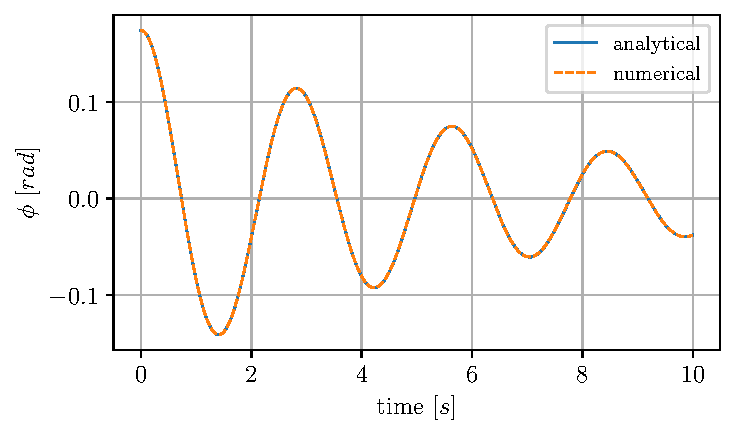
\includegraphics[width = 0.5\textwidth]{figures/analytical_numerical.pdf}\end{center}
        \vspace{-1cm}
        \caption{Analytical and numerical}
        \label{fig:analytical_numerical}
    \end{figure}
    
    